\documentclass[12pt,a4paper]{article} 

\usepackage{fn2kursstyle}
\usepackage[russian]{babel}
\usepackage[T2A]{fontenc} 
\usepackage[utf8]{inputenc} 
\usepackage{geometry}
\usepackage{graphicx}
\usepackage{mathtools}
\usepackage{tikz}
\usepackage{pdfpages}
\usepackage{booktabs}
\usepackage{multirow,array}
\usepackage{siunitx}
\usepackage{amsmath}
\usepackage[hidelinks]{hyperref}

\counterwithout{equation}{section}
\counterwithout{figure}{section}
\graphicspath{{../pic/}}
\frenchspacing 

\newcolumntype{C}[1]{>{\centering\arraybackslash}p{#1}}

\newcommand{\picref}[1]{рис. \ref{#1}}
\newcommand{\tabref}[1]{таблица \ref{#1}}
\newcommand{\half}{\frac{1}{2}}
\newcommand{\dhalf}{\dfrac{1}{2}}
\newcommand*{\Scale}[2][4]{\scalebox{#1}{$#2$}}

\title{КУСОЧНО-ПАРАБОЛИЧЕСКИЙ МЕТОД НА ЛОКАЛЬНОМ ШАБЛОНЕ ДЛЯ РЕШЕНИЯ ЛИНЕЙНОГО УРАВНЕНИЯ ПЕРЕНОСА}
\group{ФН2-62Б}
\author{А.\,И.~Токарев}
\supervisor{В.\,В.~Лукин}
\date{2022}

\begin{document}
    \maketitle
    \tableofcontents
    \pagebreak

    \section-{Введение}
    Одним из используемых вычислительных методов решения гиперболических уравнений является кусочно-параболический метод (с англ. Piecewise-Parabolic Method, PPM), разработанный для моделирования течения жидкостей и газов и применяемый в астрофизике [1]. Он обладает порядком аппроксимации $ O(\tau^2 + h^3) $. Несмотря на великолепную точность, данный метод имеет несколько существенных недостатков: возникновение ощутимых осцилляций на разрывных решениях; некомпактность шаблона, что усложняет проведение параллельных расчетов и определение граничных условий. 

    Целью данной курсовой работы является анализ варианта метода PPM -- кусочно-параболического метода на локальном шаблоне (PPML) [2]. Его основное отличие заключается в том, что граничные точки парабол внутри разностых ячеек определяются с предыдущего временного слоя по методу характеристик, что позволяет точно описывать разрывные решения и избегать накопления лишней диссипации.
    
    В качестве анализа будет приведено сравнение на примерах одномерных задач точности методов PPM и PPML, а также поведение решений на границах, в которых происходят разрывы.

    \newpage
    
    \section{Постановка задачи}

    Рассмотрим линейное уравнение переноса [3]:
    \begin{equation}
        \label{convection-diffusion}
      \dfrac{\partial y}{\partial t} + a \dfrac{\partial y}{\partial x} = 0.  
    \end{equation}

    Характеристикой уравнения \eqref{convection-diffusion} является множество точек $(x,t)$, удовлетворяющее уравнению:
    \begin{equation}
        \label{characteristics}
        \dfrac{dx}{dt} = a,    
    \end{equation}
    \noindent то есть множество $x-at = b$. 
    
    Вдоль характеристики выполняется следующее равенство:
    \[
        \dfrac{dy}{dt} = 0.  
    \]

    Как результат, получаем аналитическое решение уравнения \eqref{convection-diffusion} в виде: 
    \begin{equation}
        \label{exactSol}
        y(x, t) = y_0(x-at), 
    \end{equation}
    \noindent где $ y_0 $ -- начальный профиль.

    Уравнение переноса – простейший пример, применяемый для проверки алгоритма на корректность [3]. В задачах газодинамики оператор переноса является составной частью, поэтому любой численный метод для таких моделей обязан проходить проверку простейшим уравнением.

    Рассмотрим задачу Коши (начальная задача) для уравнения \eqref{convection-diffusion} -- поиск решения уравнения переноса на множестве $-\infty < x < +\infty,\, t > 0$, принимающее заданное значение в начальный момент времени $y(x,0) = y_0(x)$ [3]:
    \begin{equation}
        \label{Cauchy}
        \Scale[0.98] {
            \begin{cases}
                \,\dfrac{\partial y}{\partial t} + a \dfrac{\partial y}{\partial x} = 0, & x \in (-\infty,\, +\infty),\quad t > 0,
                \\[1em]
                \,y(x, 0) = y_0(x).
                \\
            \end{cases}
        }
    \end{equation}

    Определим сетку $\Omega_h = \{ x_i = l_1 + i h,\, i = 1 \ldots n,\, h = \frac{l_2-l_1}{n-1} \} $ -- множество узлов, где $[l_1, l_2]$ -- отрезок, на котором определена сетка; $n$~--~число узлов; $h$ -- шаг. Определим $y(x)$ ее разностным аналогом $y_i=y(x_i)$ на этой сетке. Значения $y_i$ будем соотносить с узлами сетки, а $ y_{ i + \half} = y_i^R $ и $ y_{i - \half} = y_i^L $ -- с половинными узлами.

    Определив решения $y_i$ в момент времени $ t_j $, можно вычислить $ \hat y_i $ на следующем временном слое $ t_{j+1} $, применив интегро-интерполяционный метод к уравнению переноса в прямоугольнике $ \bigl[ x_{i-\half}, x_{i+\half} \bigr] \times [t_j, t_{j+1}] $: 
    \[
        \int \limits_{x_{i-\half}}^{x_{i+\half}} \int \limits_{t_j}^{t_{j+1}} \dfrac{ \partial y(x, t) }{ \partial t } \, dt \, dx \,\, + \int \limits_{t_j}^{t_{j+1}} \int \limits_{x_{i-\half}}^{x_{i+\half}} a \dfrac{ \partial y(x,t) }{ \partial x } \, dx \, dt \,\, = \int \limits_{x_{i-\half}}^{x_{i+\half}} \int \limits_{t_j}^{t_{j+1}} 0 \, dt \, dx \, \, = 0.
    \]

    Рассмотрим интегралы в левой части по отдельности: 
    \[
        \Scale[0.98] {
            \begin{split}
                \int \limits_{x_{i-\half}}^{x_{i+\half}} \int \limits_{t_j}^{t_{j+1}} \dfrac{ \partial y(x, t) }{ \partial t } \, dt \, dx \,\, &= \int \limits_{x_{i-\half}}^{x_{i+\half}} \Bigl[ y(x, t_{j+1}) - y(x, t_j)  \Bigr] \, dx = h \Bigl[ \dfrac{1}{h} \int \limits_{x_{i-\half}}^{x_{i+\half}} y(x, t_{j+1}) \, dx \,\,  -  \\ 
                &- \dfrac{1}{h} \int \limits_{x_{i-\half}}^{x_{i+\half}} y(x, t_j) \, dx \Bigr] = h ( \overline y(x_i, t_{j+1}) - \overline y(x_i, t_j) ) = h( \hat y_i - y_i).
            \end{split}
        }
    \]

    Воспользуемся особенностью переноса значений по характеристикам для интеграла, подинтегральная функция которого является потоком (\picref{fig:flow_visual}):
    \[
        \begin{split}
            \int \limits_{t_j}^{t_{j+1}} \int \limits_{x_{i-\half}}^{x_{i+\half}} a \dfrac{ \partial y(x,t) }{ \partial x } \, dx \, dt \,\, &= \int \limits_{t_j}^{t_{j+1}} a \bigl( y(x_{i+\half}, t) - y(y_{x-\half}, t) \bigr) \, dt \,\, =  \int \limits_{x_{i+\half}-a\tau}^{x_{i+\half}} a y(x, t_j) \, dt \,\, - \\
            &- \int \limits_{x_{i-\half}-a\tau}^{x_{i-\half}} a y(x, t_j) \, dt = a\tau\bigl( a \overline y_{i+\half} - a \overline y_{i-\half} \bigr).
        \end{split}
    \]

    Объединяя оба интеграла получаем:
    \begin{equation}
        \begin{split}
            h ( \hat y_i - y_i) &+ a\tau\bigl( a \overline y_{i+\half} - a \overline y_{i-\half} \bigr) = 0 \,\, \Rightarrow \,\, \hat y_i = y_i - \dfrac{ a\tau }{ h } \Bigl( a \overline y_{i+\half} - a \overline y_{i-\half} \Bigr).
        \end{split}
        \label{center}
    \end{equation}

    Таким образом, используя формулу \eqref{center}, мы можем переносить средние значения ячеек.

    \pagebreak

    \begin{figure}[h]
        \centering
        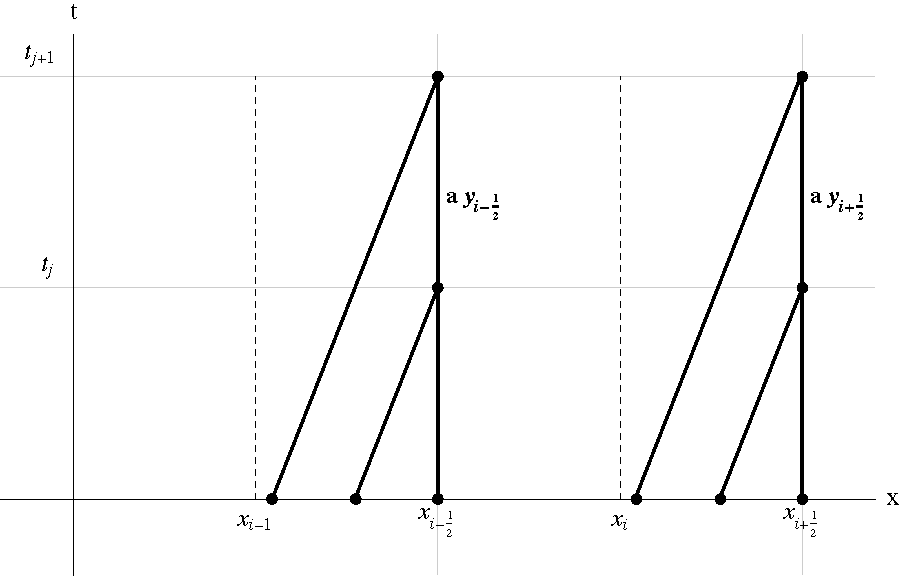
\includegraphics[width=0.897\textwidth]{flow_visual.pdf}
        \caption{Интегрирование потока по пространству, вместо времени}
        \label{fig:flow_visual}
    \end{figure}

    \section{Методы решения}
    \begin{figure}[h]
        \centering
        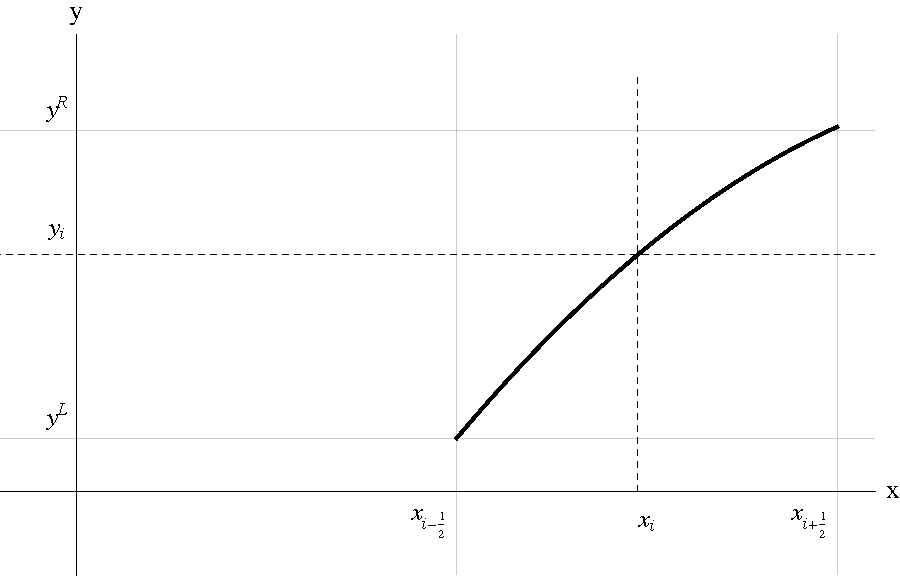
\includegraphics[width=\textwidth]{ppm_visual.pdf}
        \caption{Парабола внутри разностной ячейки}
        \label{fig:ppm_visual}
    \end{figure}

    Основная идея рассматриваемых методов заключается в аппроксимации функции $y(x)$ параболой (\picref{parabolic_eq}) на отрезках вида $ [x_{i-\half}, x_{i+\half}] $ [1]:
    \begin{equation}
    \begin{split}
        \label{parabolic_eq}
        &y(x) = y_i^L + \xi(\Delta y_i + y_i^{(6)}(1 - \xi)), \quad \xi = (x - x_{i-\half})h^{-1}, \quad  \Delta y_i = y_i^R-y_i^L, \\
        &y_i^{(6)} = 6\Bigl[ y_i - \half(y_i^R + y_i^L)\Bigr], \quad x \in [x_{i-\half}, x_{i + \half}].
    \end{split}
    \end{equation}

    Выражение \eqref{parabolic_eq} является квадратурной формулой для соотнешния:
    \[
        y(x_i) = \dfrac{1}{h} \displaystyle \int\limits_{x_{i-\half}}^{x_{i+\half}} y(\chi) d\chi.
    \]

   Значение функции $ y(x) $ на границах при условиях гладкости и отсутствия экстремумов принадлежит отрезкам:
   \begin{equation}
        \label{ppm_boundary}
        y_{i-\half} \in [y_{i-1}, y_i], \qquad y_{i+\half} \in [y_i, y_{i+1}].
   \end{equation}

   \subsection{Кусочно-параболический метод. PPM}

   Первым шагом ищем значение $y_{i+\half}$ интерполяционной процедурой четвертого порядка, в результате получаем значения:
   \[
        y_i^R = y_{i+1}^L = y_{i+\half} = \dhalf(y_i + y_{i+1}) - \dfrac{1}{6}(\delta y_{i+1} - \delta y_i),
   \] 
   \noindent где 
   \[
        \delta y_i = \dhalf(y_{i+1} + y_{i-1}).
   \]

    Чтобы обеспечить монотонность решения и выполнить условие \eqref{ppm_boundary}, значения $ \delta y_i $ нужно заменить на 
    \[
        \Scale[0.95] {
            \delta_m y_i = 
            \begin{cases}
                \min(|\delta y_i|,\, 2|y_i - y_{i-1}|,\, 2|y_{i+1} - y_i|)\cdot \text{sign}(\delta y_i), & (y_{i+1} - y_i)(y_i - y_{i-1}) > 0, \\
                0, \quad (y_{i+1} - y_i)(y_i - y_{i-1}) \leq 0.
            \end{cases}  
        }
    \]

    \pagebreak

    В областях немонотонного решения $ y(x) $ следует переопределять значения $ y_i^L,\, y_i^R $. При этом возможны два сценария:
    \begin{itemize}
        \item $ y_i $ является локальным экстремумом, тогда на всем отрезке $ [x_{i-\half}, x_{i+\half}] $ функция $ y(x) $ должна быть постоянной, а значит:
        \begin{equation}
            \label{local_sup}
            y_i^L = y_i^R = y_i, \quad (y_{i+1} - y_i)(y_i - y_{i-1}) \leq 0;
        \end{equation}
                
        \item $ y_i $ лежит слишком близко к границе -- при условии $|\Delta y_i| < | y_i^{(6)} |$ парабола может иметь экстремум внутри разностной ячейки. В этом случае $ y_i^L $ и $ y_i^R $ должны быть выбраны так, чтобы сдвинуть его к границам:
        \begin{equation}
            \label{boundary_sup}
            \begin{split}
                y_i^L = 3y_i -2y_i^R, &\quad \Delta y_i \cdot y_i^{(6)} > (\Delta y_i)^2, \\
                y_i^R = 3y_i -2y_i^L, &\quad \Delta y_i \cdot y_i^{(6)} < -(\Delta y_i)^2.
            \end{split}  
        \end{equation}
    \end{itemize}

    После всех проделанных операция функцию $y(x)$ можно считать определенной на сетке $\Omega_h$ [1, 2]. 
    
    Cреднее значение данной функции на отрезке $ [x_{i+\half}-\alpha, x_{i+\half}], (\alpha > 0) $ задается формулой, полученной путем аналитического интегрирования \eqref{parabolic_eq}:
    \begin{equation}
        \label{average_positive}
        \overline y_{i+\half}^L(\alpha) = \dfrac{1}{\alpha} \displaystyle \int\limits_{x_{i+\half}-\alpha}^{x_{i+\half}} y(x) dx = y_i^R - \dfrac{\alpha}{2h}\Bigl[ \Delta y_i - \Bigl( 1 - \dfrac{2 \alpha}{3h} \Bigr)y_i^{(6)} \Bigr],
    \end{equation}
    \noindent а на отрезке $ [x_{i+\half}, x_{i+\half}+\alpha], (\alpha > 0)$:
    \begin{equation}
        \label{average_negative}
        \overline y_{i+\half}^R = \dfrac{1}{\alpha} \displaystyle \int\limits_{x_{i+\half}}^{x_{i+\half}+\alpha} y(x) dx = y_{i+1}^L  + \dfrac{\alpha}{2h} \Bigl[\Delta y_{i+1} + \Bigl( 1 - \dfrac{2\alpha}{3h} \Bigr) y_{i+1}^{(6)} \Bigr].
    \end{equation}

    \subsection{Кусочно-параболический метод на локальном шаблоне. PPML}

    Интерполяционная процедура четвертого порядка, применяемая для переопределения граничных узлов, сглаживает разрывные решения $y(x)$. Чтобы обойти данное ограничение, можно определять $ y_i^L $ и $ y_i^R $ с помощью переноса значения на параболе с предыдущего шага по времени вдоль характеристики линейного уравнения переноса \eqref{convection-diffusion}. Для ясности  будем рассматривать правую границу $y_i^R = y_{i+\half}$. Для того, чтобы вычислить ее на следующем временном слое $ t_{j+1} = t_j + \tau$, необходимо двигаться от точки $ x_{i+\half} $ со значением $ y_{i+\half} $ вдоль характеристики до предыдущего момента времени $ t_j $:
    \begin{enumerate}
        \item $ a > 0 $, следовательно
        \begin{equation}
            \label{ppml_boundary}
            \begin{split}
                &y_{i+\half}(t_{j+1}) = y_i^R(t_{j+1}) = y_i^L(t_j) + \xi(\Delta y_i(t_j) + y_i^{(6)}(t_j)(1-\xi)), \\[0.7em]
                &\xi = 1 -  \dfrac{a \tau}{h},
            \end{split}
        \end{equation}
        \noindent что соответствует красной точке на \picref{fig:ppml_visual}.

        \item $ a < 0 $, следовательно
        \[
            \begin{split}
                &y_{i+\half}(t_{j+1}) = y_i^R(t_{j+1}) = y_{i+1}^L(t_j) + \xi(\Delta y_{i+1}(t_j) + y_{i+1}^{(6)}(t_j)(1-\xi)), \\[0.7em]
                &\xi = -\dfrac{a \tau}{h},
            \end{split}  
        \]
        \noindent что соответствует синей точке на \picref{fig:ppml_visual}.
    \end{enumerate}

    \begin{figure}[h]
        \centering
        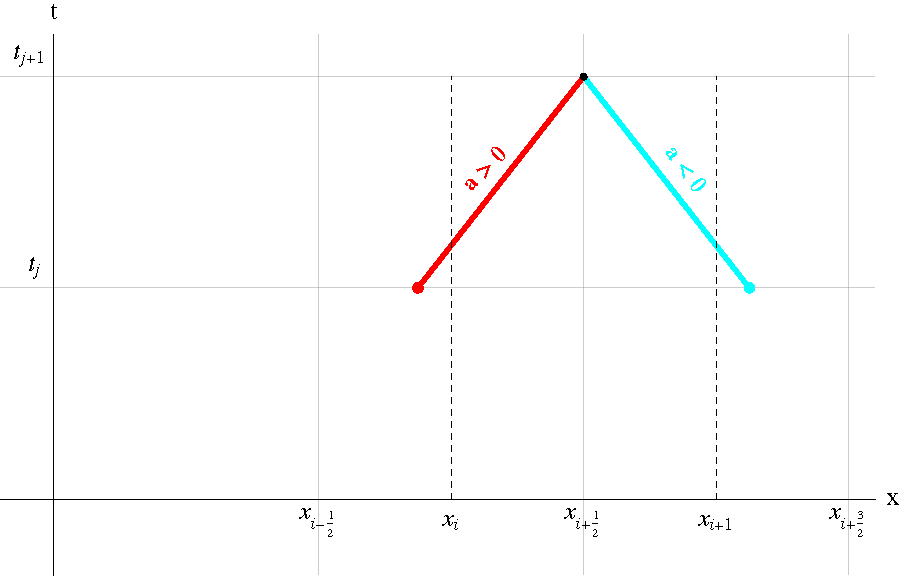
\includegraphics[width=0.93\textwidth]{ppml_visual.pdf}
        \caption{Перенос значений в граничных точках вдоль характеристик в методе PPML}
        \label{fig:ppml_visual}
    \end{figure}

    Алгоритм \eqref{ppml_boundary} реализован на локальном шаблоне, то есть для получения граничных точкек при переходе на следующий временной слой не нужно использовать информацию с соседних ячеек. Нахождение среднего значения на отрезке \eqref{average_positive}, \eqref{average_negative} и смещение экстремума \eqref{local_sup}, \eqref{boundary_sup} производятся аналогично [2].


    \subsection{Потоки и усредненное значение на отрезке}

    При возникновении разрыва на границе двух смежных ячеек в точке $ x_{i+\half} $ возникает некоторое усредненное состояние $ y^\star(x_{i+\half}, t) $. Одномерное уравнение переноса имеет всего одну характеристику, поэтому его решение в момент времени $ t = t_{j+1} $ будет определяться:
    \begin{enumerate}
        \item При $ a > 0 $ усреднением по пространствунному интервалу $ [x_{i+\half}-a \tau, x_{i+\half}] $ со значением $ y^\star(x_{i+\half}, t_{j+1}) = \overline y_{i+\half}^L(a \tau) $;
        
        \item При $ a < 0 $ -- усреднением по интервалу $ [x_{i+\half} \tau, x_{i+\half}+a \tau] $ со значением $ y^\star(x_{i+\half}, t_{j+1}) = \overline y_{i+\half}^R(-a \tau) $.
    \end{enumerate}

    Поток на границе смежных ячеек в задаче Римана определяется по формуле:
    \begin{equation}
        \label{boundary_flow}
        \begin{split}
            &F_{i+\half} = \dfrac{1}{\tau} \displaystyle \int\limits_{t_j}^{t_{j+1}} F(y^\star(x_{i+\half}, t))dt = a^+ y_{i+\half}^L + a^- y_{i+\half}^R, \\[0.5em]
            &a^+ = \max(0, a), \quad a^- = \min(a, 0).
        \end{split}
    \end{equation}

    \section{Анализ и сравнение}

    Оценивать решение будем по норме ошибки в пространствах $ C,\, L_1,\, L_2\colon $
    \[
        \|z\|_{C} = \max_{\Omega_h \times [0, T]} |z|, \quad z = |y(x,t)-y_h(x,t)|;
    \]
    \[
        \|z\|_{L_1} = \int\limits_{0}^{T}\int\limits_{\Omega_h} |z|\, dx dt, \quad z = |y(x,t)-y_h(x,t)|;
    \]
    \[
        \|z\|_{L_2} = \Biggl( \int\limits_{0}^{T}\int\limits_{\Omega_h} z^2\, dx dt \Biggr)^{\tfrac{1}{2}}, \quad z = |y(x,t)-y_h(x,t)|,
    \]
    \noindent для методов актуальна сходимость по норме $ L_2 $.

    Рассмотрим несколько начальных профилей [3] и проанализируем точность каждого из методов в различных сценариях. Примем $ l = 200,\, l_1 = 10,\, l_2 = 30,$
    \noindent $ l_{11} = \frac{50}{3},\, l_{22} = \frac{70}{3},\, l_{12} = 20,\, T = 200,\, h = 1,\, a = 1$.

    \subsection{Анализ точного вычисления граничных и серединных узлов}

    Рассмотрим, какой прирост точности дает метод PPML при числе Куранта $ \sigma = 1 $. В качестве иллюстрации приведем кусочно-линейный профиль -- правый треугольник.

    Правый треугольник задается уравнением:
    \[
        \begin{cases}
            y_0(x) = 0, & x < l_1; \\
            y_0(x) = \dfrac{l_2 - x}{l_2 - l_1}, & x \in [l_1, l_2]; \\ 
            y_0(x) = 0, & x > l_2.
        \end{cases}
    \]

    На \picref{fig:ppm_rightTriangle_1} показано численное решение, полученное путем применения метода PPM. 

    Заметим, что на концах треугольников происходит разрыв решений в ячейках $ y_i^L,\, y_i,\, y_i^R $, поэтому, например, вычисление нормы в пространтсве $C[a,b]$ неприменимо для данных методов, потому что ее значение не будет уменьшаться при измельчении шага на кусочно-линейных графиках.

    Из таблицы \refeq{table:ltPPM} можно сделать вывод о порядке точности метода PPM для профиля "правый треугольник":
    \[
        \begin{split}
        &\text{В пространстве $L_1$}\colon \, \psi_{h}^{(2)} = 4.05 \approx 4;\,\, \psi_{\tau}^{(2)} = 1.995 \approx 2.
        \\[0.5em]
        & \text{В пространстве $L_2$}\colon \, \psi_{h}^{(2)} = 2.003 \approx 2;\,\, \psi_{\tau}^{(2)} = 1.41.
        \end{split}
    \]
    \pagebreak


     \begin{figure}[h]
        \centering
        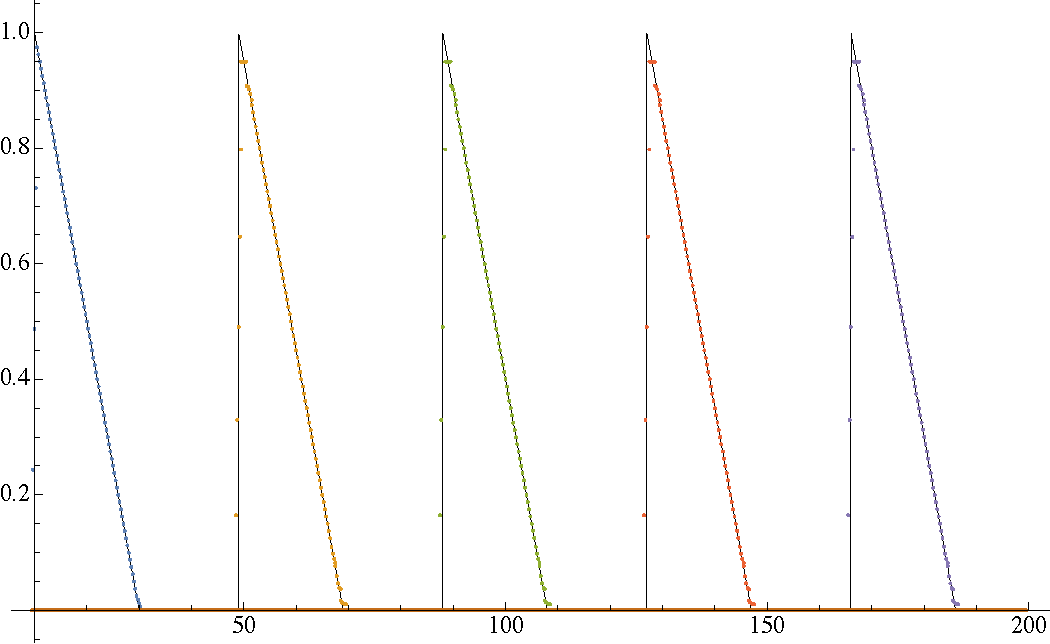
\includegraphics[width=\textwidth]{sigma=1./advectionPPM_rightTriangle.pdf}
        \caption{Правый треугольник для PPM при $ \sigma = 1 $}
        \label{fig:ppm_rightTriangle_1}
    \end{figure}

    \begin{table}[h]
        \centering
        \caption{Нормы ошибок для правого треугольника в методе PPM}
        \label{table:ltPPM}
        \scalebox{0.75} {
            \begin{tabular}{|*{10}{C{.58in}|}}
                \noalign{\vskip 2mm}
                \hline
                & \multicolumn{3}{c|}{$h=1$} & \multicolumn{3}{c|}{$h=0.5$} & \multicolumn{3}{c|}{$h=0.25$} \\
                \cline{2-10}
                & $\tau=1$ & $\tau=0.5$ & $\tau=0.25$ & $\tau=1$ & $\tau=0.5$ & $\tau=0.25$ & $\tau=1$ & $\tau=0.5$ & $\tau=0.25$ 
                \\ \hline
                $\| \cdot \|_{C}$ & 0.5125 & 0.58 & 0.65 & 0.506 & 0.61 & 0.695 & 0.503 & 0.613 & 0.696
                \\ \hline
                $\| \cdot \|_{L_1}$ & 1.038 & 0.519 & 0.26 & 0.255 & 0.13 & 0.064 & 0.063 & 0.0315 & 0.0158
                \\ \hline
                $\| \cdot \|_{L_2}$ & 0.622 & 0.44 & 0.311 & 0.309 & 0.22 & 0.154 & 0.154 & 0.1087 & 0.077
                \\ \hline
            \end{tabular}
        }
    \end{table}

    На \picref{fig:ppml_rightTriangle_1} показано решение, полученное с применением метода PPML. На концах треугольников параболы в каждой разностной ячейке передают значения гораздо точнее, чем в методе PPM.

    Скорость стремления нормы к нулю (\tabref{table:ltPPML}) практически идентична методу PPM, однако визуально график больше приближен к точному решению. Оценим порядок точности метода PPML:
    \[
        \begin{split}
        &\text{В пространстве $L_1$}\colon \, \psi_{h}^{(2)} \approx 4;\,\, \psi_{\tau}^{(2)} \approx 2.
        \\[0.5em]
        & \text{В пространстве $L_2$}\colon \, \psi_{h}^{(2)}\approx 2;\,\, \psi_{\tau}^{(2)} \approx 1.4.
        \end{split}
    \]

    \pagebreak

    \begin{figure}[h]
        \centering
        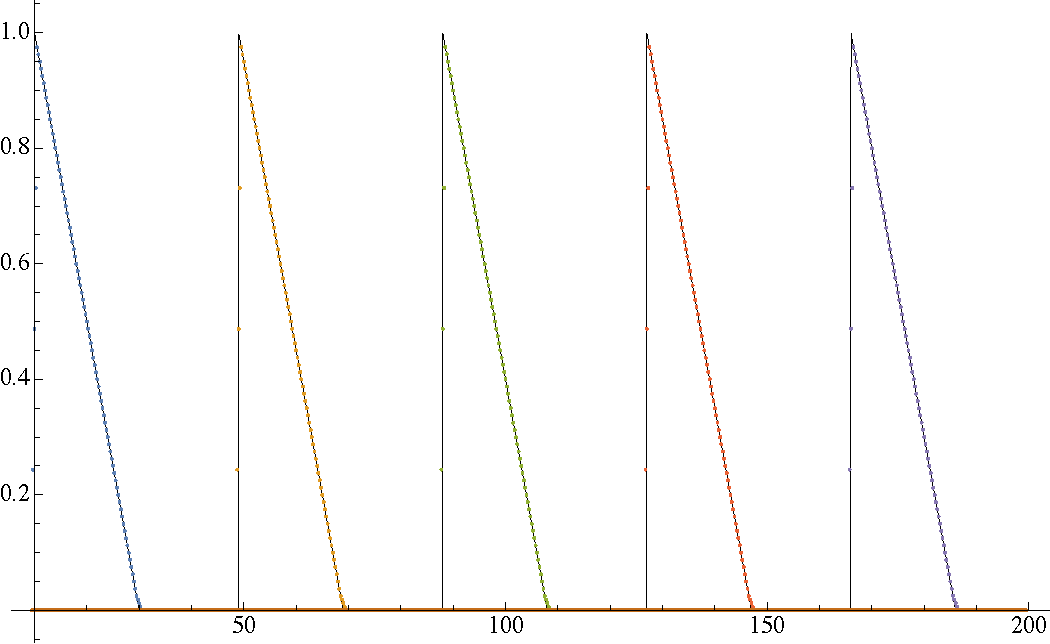
\includegraphics[width=\textwidth]{sigma=1./advectionPPML_rightTriangle.pdf}
        \caption{Правый треугольник для PPML при $ \sigma = 1 $}
        \label{fig:ppml_rightTriangle_1}
    \end{figure}

    \begin{table}[h]
        \centering
        \caption{Нормы ошибок для правого треугольника в методе PPML}
        \label{table:ltPPML}
        \scalebox{0.75} {
            \begin{tabular}{|*{10}{C{.58in}|}}
                \noalign{\vskip 2mm}
                \hline
                & \multicolumn{3}{c|}{$h=1$} & \multicolumn{3}{c|}{$h=0.5$} & \multicolumn{3}{c|}{$h=0.25$} \\
                \cline{2-10}
                & $\tau=1$ & $\tau=0.5$ & $\tau=0.25$ & $\tau=1$ & $\tau=0.5$ & $\tau=0.25$ & $\tau=1$ & $\tau=0.5$ & $\tau=0.25$ 
                \\ \hline
                $\| \cdot \|_{C}$ & 0.5125 & 0.5039 & 0.5544 & 0.50625 & 0.502 & 0.5487 & 0.5031 & 0.5001 & 0.5458
                \\ \hline
                $\| \cdot \|_{L_1}$ & 1.0375 & 0.5187 & 0.2593 & 0.255 & 0.1273 & 0.0637 & 0.063 & 0.03154 & 0.01577
                \\ \hline
                $\| \cdot \|_{L_2}$ & 0.6228 & 0.4404 & 0.3114 & 0.3087 & 0.2183 & 0.1544 & 0.1537 & 0.1087 & 0.0768  
                \\ \hline
            \end{tabular}
        }
    \end{table}

    \pagebreak

    \subsection{Анализ кусочно-линейного графика при уменьшенном числе Куранта }

    Рассмотрим $ \sigma = 0.8 $, в качестве примера рассмотрим профиль "зуб":

    \[
        y_0(x) = \begin{cases}
            -\dfrac{2(x-l_1)}{3(l_{11}-l_1)} + 1, & x \in [l_1, l_{11}), \\[0.7em]
               \dfrac{1}{3}, & x \in [l_{11}, l_{22}],
               \\[0.7em]
           \dfrac{2(x-l_{2})}{3(l_2 - l_{22})} + 1, & x \in (l_{22}, l2].
       \end{cases}   
    \]

    На \picref{fig:ppm_tooth_08} заметна значительная диссипация и неодинаковые высоты на зубцах. 

    \begin{figure}[h]
        \centering
        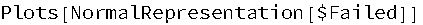
\includegraphics[width=\textwidth]{sigma=0.8/advectionPPM_tooth.pdf}
        \caption{Зуб для PPM при $ \sigma = 0.8 $}
        \label{fig:ppm_tooth_08}
    \end{figure}

    Тем не менее, несмотря на диссипацию, сходимость по норме $ L_2 $ сохраняется (\tabref{table:toothPPM}). Точность метода PPM для профиля "зуб":
    \[
        \begin{split}
        &\text{В пространстве $L_1$}\colon \, \psi_{h}^{(2)} \approx 4;\,\, \psi_{\tau}^{(2)} \approx 2.
        \\[0.5em]
        & \text{В пространстве $L_2$}\colon \, \psi_{h}^{(2)}\approx 2;\,\, \psi_{\tau}^{(2)} \approx 1.4.
        \end{split}
    \]

    \begin{table}[h]
        \centering
        \caption{Нормы ошибок для профиля "зуб" в методе PPM}
        \label{table:toothPPM}
        \scalebox{0.75} {
            \begin{tabular}{|*{10}{C{.58in}|}}
                \noalign{\vskip 2mm}
                \hline
                & \multicolumn{3}{c|}{$h=1$} & \multicolumn{3}{c|}{$h=0.5$} & \multicolumn{3}{c|}{$h=0.25$} \\
                \cline{2-10}
                & $\tau=1$ & $\tau=0.5$ & $\tau=0.25$ & $\tau=1$ & $\tau=0.5$ & $\tau=0.25$ & $\tau=1$ & $\tau=0.5$ & $\tau=0.25$ 
                \\ \hline
                $\| \cdot \|_{C}$ & 0.525 & 0.84 & 0.754 & 0.5125 & 0.8375 & 0.7501 & 0.50625 & 0.835 & 0.7494 
                \\ \hline
                $\| \cdot \|_{L_1}$ & 2.1 & 1.05 & 0.525 & 0.5125 & 0.26 & 0.13 & 0.127 & 0.0633 & 0.032
                \\ \hline
                $\| \cdot \|_{L_2}$ & 0.9 & 0.63 & 0.45 & 0.44 & 0.311 & 0.22 & 0.22 & 0.154 & 0.11
                \\ \hline
            \end{tabular}
        }
    \end{table}

    Метод PPML (\picref{fig:ppml_tooth_08}) характеризиуется менее выраженной диссипацией и более ровными "горбами". 

    \begin{figure}[h]
        \centering
        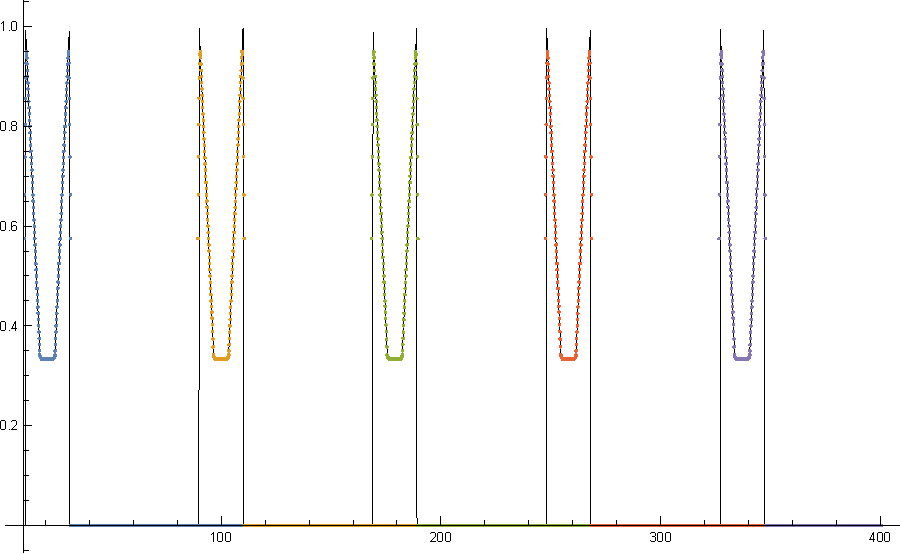
\includegraphics[width=\textwidth]{sigma=0.8/advectionPPML_tooth.pdf}
        \caption{Зуб для PPML при $ \sigma = 0.8 $}
        \label{fig:ppml_tooth_08}
    \end{figure}

    Помимо этого, анализ норм ошибок для метода PPML также показывает повышенную точность во всех рассматриваемых пространствах (\tabref{table:toothPPML}). Точность метода остается такой же, как и во всех предыдущих случаях: 
    \[
        \begin{split}
        &\text{В пространстве $L_1$}\colon \, \psi_{h}^{(2)} \approx 4;\,\, \psi_{\tau}^{(2)} \approx 2.
        \\[0.5em]
        & \text{В пространстве $L_2$}\colon \, \psi_{h}^{(2)}\approx 2;\,\, \psi_{\tau}^{(2)} \approx 1.4.
        \end{split}
    \]

    \begin{table}[h]
        \centering
        \caption{Нормы ошибок для профиля "зуб" в методе PPML}
        \label{table:toothPPML}
        \scalebox{0.75} {
            \begin{tabular}{|*{10}{C{.58in}|}}
                \noalign{\vskip 2mm}
                \hline
                & \multicolumn{3}{c|}{$h=1$} & \multicolumn{3}{c|}{$h=0.5$} & \multicolumn{3}{c|}{$h=0.25$} \\
                \cline{2-10}
                & $\tau=1$ & $\tau=0.5$ & $\tau=0.25$ & $\tau=1$ & $\tau=0.5$ & $\tau=0.25$ & $\tau=1$ & $\tau=0.5$ & $\tau=0.25$ 
                \\ \hline
                $\| \cdot \|_{C}$ & 0.525 & 0.6437 & 0.6347 & 0.5125 & 0.6343 & 0.6262 & 0.50625 & 0.6297 & 0.6219
                \\ \hline
                $\| \cdot \|_{L_1}$ & 2.1 & 1.049 & 0.5249 & 0.5125 & 0.2563 & 0.1281 & 0.1265 & 0.0633 & 0.03164 
                \\ \hline
                $\| \cdot \|_{L_2}$ & 0.895 & 0.633 & 0.4478 & 0.4403 & 0.3113 & 0.2202 & 0.2183 & 0.1544 & 0.10916
                \\ \hline
            \end{tabular}
        }
    \end{table}

    \pagebreak

    \subsection{Анализ методов на непрерывном графике}

    Пусть $ \sigma = 0.5 $. Сравним методы на примере профиля:
    \[
        y_0(x) = \dfrac{1}{2} - \dfrac{1}{2} \cos\Bigl(\dfrac{2 \pi}{l_2 - l_1}(x-l_1)\Bigr).
    \]

    Как и следовало ожидать, несмотря на гладкость профиля, диссипация в случае метода PPM (\picref{fig:ppm_cos_05}), ровно как и в методе PPML (\picref{fig:ppml_cos_05}) остается, хотя и менее выраженная. 

    \begin{figure}[h]
        \centering
        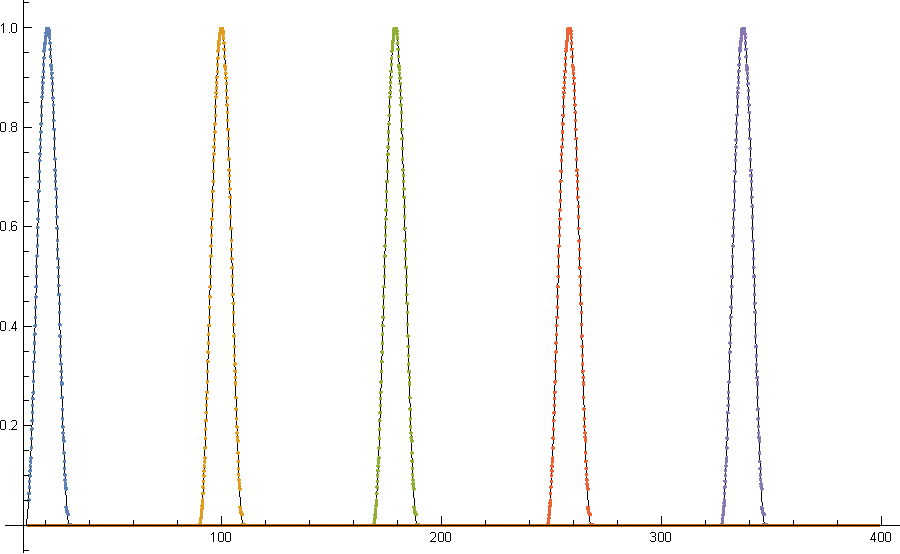
\includegraphics[width=\textwidth]{sigma=0.5/advectionPPM_cos.pdf}
        \caption{Косинус для PPM при $ \sigma = 0.5 $}
        \label{fig:ppm_cos_05}
    \end{figure}

    График сохраняет свою гладкость, однако происходят заметные отклонения от точного решения в окрестностях оснований профилей. Хотя таблицы с погрешностями решений \ref{table:cosPPM}, \ref{table:cosPPML} показывают достаточно хороший результат для обоих методов, все же нельзя не отметить, что PPML стабильнее передает точное решение, а также обладает меньшей диссипацией. 

    \begin{table}[h]
        \centering
        \caption{Нормы ошибок для косинуса в методе PPM}
        \label{table:cosPPM}
        \scalebox{0.75} {
            \begin{tabular}{|*{10}{C{.58in}|}}
                \noalign{\vskip 2mm}
                \hline
                & \multicolumn{3}{c|}{$h=1$} & \multicolumn{3}{c|}{$h=0.5$} & \multicolumn{3}{c|}{$h=0.25$} \\
                \cline{2-10}
                & $\tau=1$ & $\tau=0.5$ & $\tau=0.25$ & $\tau=1$ & $\tau=0.5$ & $\tau=0.25$ & $\tau=1$ & $\tau=0.5$ & $\tau=0.25$ 
                \\ \hline
                $\| \cdot \|_{C}$ & 0.078 & 0.244 & 0.242 & 0.039 & 0.11 & 0.156 & 0.0196 & 0.044 & 0.06 
                \\ \hline
                $\| \cdot \|_{L_1}$ & 0.195 & 0.098 & 0.048 & 0.0245 & 0.012 & 0.006 & 0.003 & 0.0015 & 0.00077 
                \\ \hline
                $\| \cdot \|_{L_2}$ & 0.028 & 0.02 & 0.014 & 0.005 & 0.0035 & 0.00245 & 0.00089 & 0.0006 & 0.00044
                \\ \hline
            \end{tabular}
        }
    \end{table}


    \begin{figure}[h]
        \centering
        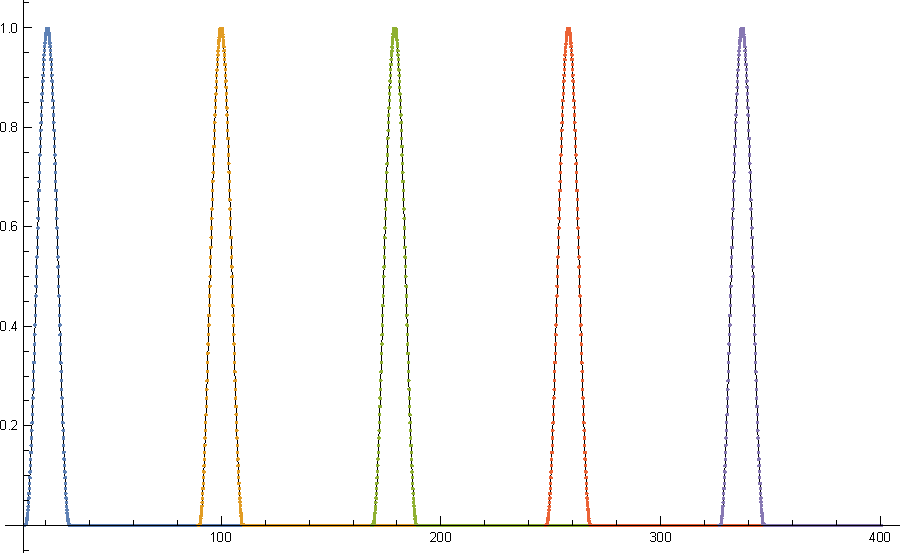
\includegraphics[width=0.8\textwidth]{sigma=0.5/advectionPPML_cos.pdf}
        \caption{Косинус для PPML при $ \sigma = 0.5 $}
        \label{fig:ppml_cos_05}
    \end{figure}

    \begin{table}[h]
        \centering
        \caption{Нормы ошибок для косинуса в методе PPML}
        \label{table:cosPPML}
        \scalebox{0.75} {
            \begin{tabular}{|*{10}{C{.58in}|}}
                \noalign{\vskip 2mm}
                \hline
                & \multicolumn{3}{c|}{$h=1$} & \multicolumn{3}{c|}{$h=0.5$} & \multicolumn{3}{c|}{$h=0.25$} \\
                \cline{2-10}
                & $\tau=1$ & $\tau=0.5$ & $\tau=0.25$ & $\tau=1$ & $\tau=0.5$ & $\tau=0.25$ & $\tau=1$ & $\tau=0.5$ & $\tau=0.25$ 
                \\ \hline
                $\| \cdot \|_{C}$ & 0.00615 & 0.0479 & 0.0576 & 0.00154 & 0.0158 & 0.01859 & 0.00039 & 0.00515 & 0.00599
                \\ \hline
                $\| \cdot \|_{L_1}$ & 0.19475 & 0.09738 & 0.0487 & 0.02449 & 0.01225 & 0.0061 & 0.00306 & 0.00153 & 0.00076
                \\ \hline
                $\| \cdot \|_{L_2}$ & 0.0277 & 0.01958 & 0.01384 & 0.005 & 0.00351 & 0.00248 & 0.00088 & 0.00059 & 0.00044
                \\ \hline
            \end{tabular}
        }
    \end{table}

    \pagebreak

    \section-{Заключение}

    Рассмотрен кусочно-параболический метод на локальном шаблоне. Выбор в пользу использования решений с предыдущего временного слоя, вместо интерполяционной процедуры, оказался удачным, так как обеспечивает более точное решение и уменьшенную диссипацию. Метод PPML протестирован на ряде примеров, рассмотренных с различными шагами, числами Куранта и профилями. Точность оценивалась на основе норм разности между точным и численным решениям в пространствах $ C,\, L_1,\, L_2 $. В пространствах $L_1, \, L_2$ PPML оказался точнее во всех случаях. Однако в пространстве $C$ результат нельзя интерпретировать однозначно. Но как уже отмечалось, актуальной является сходимость нормы ошибки в $L_2$.

    \newpage

    \begin{thebibliography}{9}
  
        \bibitem{Corella} Corella P., Woodward P. The piecewise parabolic method for gas-dynamical simulations // J. Comput. Phys. $1984$. -- P. $174-201$.
  
        \bibitem{Article} М.\,В.\,Попов, С.\,Д.\,Устюгов. Кусочно-параболический метод на локальном шаблоне для задач газовой динамики // Ж. вычисл. матем. и матем. физ., $2007$. -- C. $2056-2060$.
  
        \bibitem{Galanin} Галанин М. П., Савенков Е. Б. Методы численного анализа математических моделей. -- М. : Изд-во МГТУ им. Н. Э. Баумана, 2018. -- 591~с.

        \bibitem{Samarsky} А.\,А.\,Самарский, Ю.\,П.\,Попов. Разностные методы решения задач газовой динамики. -- M.: Наука. Гл. ред. физ. мат. лит., $1992$. -- $424$ с.

        \bibitem{Kulikovsky} А.\,Г.\,Куликовский, Н.\,В.\,Погорелов, А.\,Ю.\,Семенов. Математические вопросы численного решения гиперболических систем уравнений. -- М.: ФИЗМАТЛИТ, $2001$. -- $608$ с.
  
    \end{thebibliography}

\end{document}